\documentclass[12pt]{article}
\usepackage[utf8]{inputenc}
\usepackage[total={19cm,22cm},centering]{geometry} %define tamaño para imprimir hoja
\usepackage{wrapfig}
\usepackage{tikz}
\usepackage{schemabloc}
\usepackage{graphicx}
\usepackage{amssymb}
\usepackage{amsmath}
\usepackage{mathrsfs}
\usepackage{tcolorbox}
\tcbuselibrary{theorems}
\usepackage{color}
\usepackage[europeanresistors, americaninductors]{circuitikz}
\usetikzlibrary{calc}
\usetikzlibrary{patterns}

\usepackage{fancyhdr}
\pagestyle{fancy}
\lhead[]{\textbf{Practico 2}}
\rhead[]{ELN-360 E2}
\chead[]{Control 1}

\lfoot[]{UAGRM}
\rfoot[]{\number\thepage}
\cfoot[]{}
\renewcommand{\footrulewidth}{0.8pt}

\usetikzlibrary{patterns,angles,quotes}

\ctikzset{bipoles/thickness=1} %grosor elementos pasivos dos polos
%\ctikzset{bipoles/length=1.2cm} %longitud de elementos pasivos dos polos
%\tikzstyle{every node}=[font\normalsize] %Tamaño de las etiquetas
\tikzstyle{every path}=[line width=1pt, line cap=round, line join=round] %Caracteristicas linea union


%\title{Apuntes de clase}
%\author{Lima Soto Ariel Wilson}
%\date{\today}



\begin{document}

\section*{Ejercicio \# 1}
Determinar la funci\'on de transferencia, si su entrada es un
escal\'on unitario cu\'al es su sobreimpulso y su tiempo de 
estabilizaci\'on.

%Ejercicio 3 Disgrama de bloque de sistemas de control.
  \vspace{1cm}
  \renewcommand{\theenumi}{\alph{enumi}}
  \begin{enumerate}

  \item
  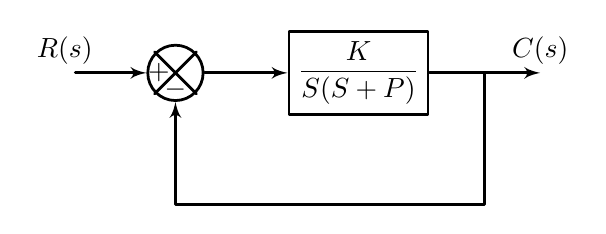
\begin{tikzpicture}
     \sbEntree{E}
     \sbCompSum[4]{sum1}{E}{}{-}{+}{}
     \sbRelier{E}{sum1}
     \sbNomLien[0.8]{E}{$R(s)$}
     \sbBlocL[3]{a}{$\dfrac{K}{S(S+P)}$}{sum1}
     \sbSortie[4]{S}{a}
     \sbRelier{a}{S}
     \sbNomLien[0.8]{S}{$C(s)$}
    \sbRenvoi[4]{a-S}{sum1}{}
     %\coordinate (A) at (16.65,0);
     %\coordinate (B) at (16.34,2.1);
     %\draw (A) |- (B);
     %\draw[-stealth] (B) -- (C)node[near end,right]{$+$};
     %\draw[-stealth] (sum.east) -- (controller.west)node[midway,above]{$e$};
     
  \end{tikzpicture}
      
  
      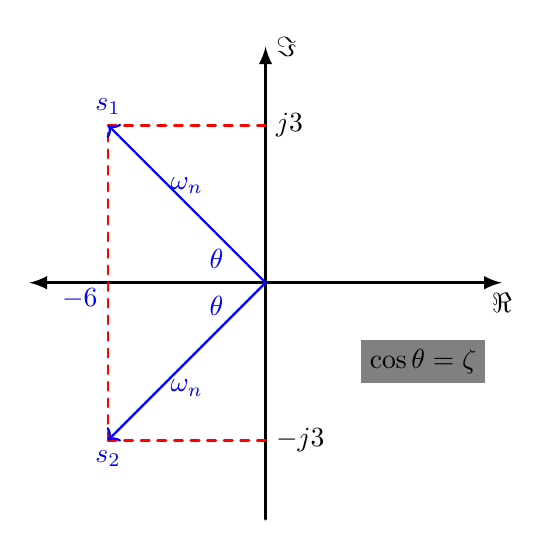
\begin{tikzpicture}
        %eje reales
        \draw[very thick,latex-latex] (-3,-1) -- (3,-1) node[below]{$\Re$};
        %eje imaginarios
        \draw[very thick,-latex] (0,-4) -- (0,2) node[right]{$\Im$};
        %polos
        \draw[dashed, red] (-2,-3) -- (-2,1);
        \draw[dashed, red] (0,-3) -- (-2,-3);
        \node[right] at (0,-3) {$-j3$};
        \node[fill=gray,text=black] at (2,-2) {$\cos{\theta}=\zeta$};
        \draw[dashed, red] (0,1) -- (-2,1);
        \node[right] at (0,1) {$j3$};
        %Wn
        \draw[thick, blue, ->] (0,-1) -- (-2,1);
        \node[above, blue] at (-1,0) {$\omega_n$};
        \node[above, blue] at (-2,1) {$s_1$};
        \draw[thick, blue, ->] (0,-1) -- (-2,-3);
        \node[below, blue] at (-1,-2.1) {$\omega_n$};
        \node[below, blue] at (-2,-3) {$s_2$};
        \node[left, blue] at (-2,-1.2) {$-6$};
        %angulo thita
        \node[left, blue] at (-0.4,-1.3) {$\theta$};
        \node[left, blue] at (-0.4,-0.7) {$\theta$};
 \end{tikzpicture}

      Se obtiene la siguiente funcion de transferencia \( \displaystyle FT=\frac{C(s)}{R(s)} = \frac{K}{s^2 + ps + K} \)

      en donde:

      \( \displaystyle K = \omega_{n}^{2}\)\\
      \( \displaystyle P = 2\zeta \omega_{n}\)

      Reemplazamos:

      \( \displaystyle \frac{C(s)}{R(s)} = \frac{\omega_{n}^{2}}{s^2 + 2\zeta \omega_{n} s + \omega_{n}^{2}} \)

      De la gr\'afica se obtiene los valores de los polos:

      C\'alculo de la frecuencia natural no amortiguada:

      \( \displaystyle \omega_n^{2}= 3^2 + 6^2 = 45 \hspace{5mm} \rightarrow \hspace{5mm} \omega_{n}=\sqrt{45} \)

      C\'alculo del coeficiente de amortiguamiento:

      \( \displaystyle \cos{\theta} = \zeta = \frac{6}{\omega_{n}} = \frac{6}{\sqrt{45}} \)

      C\'alculo de \textbf{P}:

      \( \displaystyle P = 2\zeta \omega_{n} = 2 \alpha =
      2 \left ( \frac{6}{\sqrt{45}} \right)\sqrt{45} = 12 \)

      \vspace{1cm}

    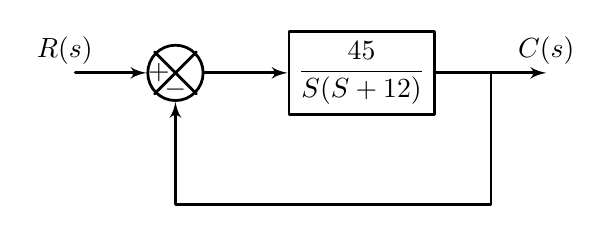
\begin{tikzpicture}
       \sbEntree{E}
       \sbCompSum[4]{sum1}{E}{}{-}{+}{}
       \sbRelier{E}{sum1}
       \sbNomLien[0.8]{E}{$R(s)$}
       \sbBlocL[3]{a}{$\dfrac{45}{S(S+12)}$}{sum1}
       \sbSortie[4]{S}{a}
       \sbRelier{a}{S}
       \sbNomLien[0.8]{S}{$C(s)$}
       \sbRenvoi[4]{a-S}{sum1}{}
     %\coordinate (A) at (16.65,0);
     %\coordinate (B) at (16.34,2.1);
     %\draw (A) |- (B);
     %\draw[-stealth] (B) -- (C)node[near end,right]{$+$};
     %\draw[-stealth] (sum.east) -- (controller.west)node[midway,above]{$e$};
     
    \end{tikzpicture}

    \vspace{1cm}


    \( \displaystyle \frac{C(s)}{R(s)} = \frac{45}{s^2 + 12s + 45} \)

    \vspace{1cm}
    C\'alculo del m\'aximo sobreimpulso:

    \( \displaystyle M_p(\%) = 100\cdot e^{- \dfrac{\zeta \pi}{\sqrt{1 - \zeta^{2}}}} \)\\
    \( \displaystyle M_p(\%) = 100\cdot e^{- \dfrac{\tfrac{6}{\sqrt{45}} \pi}{\sqrt{1 - \left ( \tfrac{6}{\sqrt{45}} \right )^{2}}}} \)\\
    \( \displaystyle M_p(\%) = 0.187 \% \)\\

    C\'alculo del tiempo de estabilizaci\'on:

    \( \displaystyle T_{s} = 4 \tau = \frac{4}{\alpha} =
    \frac{4}{\zeta \omega_{n}} = \frac{4}{\left( \dfrac{6}{\sqrt{45}}\right) \sqrt{45}} = 0.67 segundos \)


      \newpage

      \item
        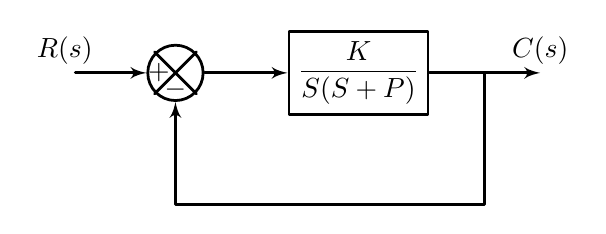
\begin{tikzpicture}
          \sbEntree{E}
          \sbCompSum[4]{sum1}{E}{}{-}{+}{}
          \sbRelier{E}{sum1}
          \sbNomLien[0.8]{E}{$R(s)$}
          \sbBlocL[3]{a}{$\dfrac{K}{S(S+P)}$}{sum1}
          \sbSortie[4]{S}{a}
          \sbRelier{a}{S}
          \sbNomLien[0.8]{S}{$C(s)$}
          \sbRenvoi[4]{a-S}{sum1}{}

        \end{tikzpicture}

        \begin{tikzpicture}
          %eje reales
          \draw[very thick,latex-latex] (-5,-1) -- (3,-1) node[below]{$\Re$};
          %eje imaginarios
          \draw[very thick,-latex] (0,-4) -- (0,2) node[right]{$\Im$};
          %polos
          \node[above, blue] at (-2,-1) {$s_1$};
          \node[circ] at (-2,-1) {};
          \node[circ] at (-4,-1) {};
          \node[below, blue] at (-2,-1) {$-3$};
          \node[above, blue] at (-4,-1) {$s_2$};
          \node[below, blue] at (-4,-1) {$-9$};
        \end{tikzpicture}

      En este caso los polos solo estan en el eje real.

    \( \displaystyle \frac{C(s)}{R(s)} = \frac{K}{s^2 + Ps + K} \)\\

    \( \displaystyle s^2 + Ps + K = (s+9)(s+3)\)\\

    \( \displaystyle s^2 + 3s + 9 = s^2 + 12s + 27 \)\\
    
    Donde $K=27$ y $P=12$.

      \vspace{1cm}

    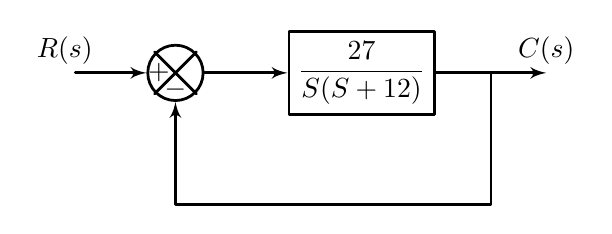
\begin{tikzpicture}
       \sbEntree{E}
       \sbCompSum[4]{sum1}{E}{}{-}{+}{}
       \sbRelier{E}{sum1}
       \sbNomLien[0.8]{E}{$R(s)$}
       \sbBlocL[3]{a}{$\dfrac{27}{S(S+12)}$}{sum1}
       \sbSortie[4]{S}{a}
       \sbRelier{a}{S}
       \sbNomLien[0.8]{S}{$C(s)$}
       \sbRenvoi[4]{a-S}{sum1}{}
     %\coordinate (A) at (16.65,0);
     %\coordinate (B) at (16.34,2.1);
     %\draw (A) |- (B);
     %\draw[-stealth] (B) -- (C)node[near end,right]{$+$};
     %\draw[-stealth] (sum.east) -- (controller.west)node[midway,above]{$e$};
     
    \end{tikzpicture}

    \vspace{1cm}


    \( \displaystyle \frac{C(s)}{R(s)} = \frac{27}{s^2 + 12s + 27} \)

    \( \displaystyle \frac{C(s)}{R(s)} = \frac{\omega_{n}^{2}}{s^2 + 2\zeta \omega_{n}s + \omega_{n}^{2}} \)
    
    \( \displaystyle \omega_{n}^{2}=27 \rightarrow \omega_{n}=\sqrt{27} \)

    \( \displaystyle 2\zeta \omega_{n}=12 \rightarrow \zeta = \frac{12}{2\omega_{n}}= \frac{12}{2\sqrt{27}} \cong 1.1547 \)

    C\'alculo de tiempo de estabilizaci\'on:

    \( \displaystyle T_{s} = 4 \tau = \frac{4}{\alpha} =
    \frac{4}{\zeta \omega_{n}} = \frac{4}{\left( \dfrac{12}{2\sqrt{27}}\right) \sqrt{27}} = 0.67 segundos \)


    \vspace{1cm}

    C\'alculo del m\'aximo sobreimpulso:

    \( \displaystyle M_p(\%) = 100\cdot e^{- \dfrac{\zeta \pi}{\sqrt{1 - \zeta^{2}}}} \)\\
    \( \displaystyle M_p(\%) = 100\cdot e^{- \dfrac{\tfrac{12}{2\sqrt{27}} \pi}{\sqrt{1 - \left ( \tfrac{12}{2\sqrt{27}} \right )^{2}}}} \)\\
    \( \displaystyle M_p(\%) = imaginario\% \)\\

      \newpage

      \item
        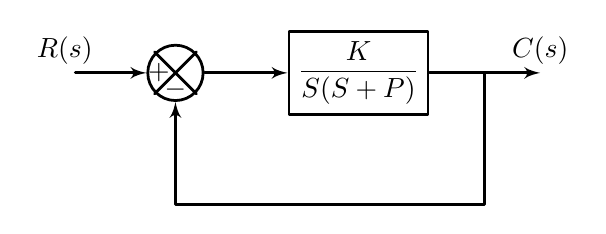
\begin{tikzpicture}
          \sbEntree{E}
          \sbCompSum[4]{sum1}{E}{}{-}{+}{}
          \sbRelier{E}{sum1}
          \sbNomLien[0.8]{E}{$R(s)$}
          \sbBlocL[3]{a}{$\dfrac{K}{S(S+P)}$}{sum1}
          \sbSortie[4]{S}{a}
          \sbRelier{a}{S}
          \sbNomLien[0.8]{S}{$C(s)$}
          \sbRenvoi[4]{a-S}{sum1}{}
        \end{tikzpicture}

        \begin{tikzpicture}
          %eje reales
          \draw[very thick,latex-latex] (-3,-1) -- (3,-1) node[below]{$\Re$};
          %eje imaginarios
          \draw[very thick,-latex] (0,-4) -- (0,2) node[right]{$\Im$};
          %polos
          \node[left, blue] at (0,1) {$s_1$};
          \node[circ] at (0,1) {};
          \node[circ] at (0,-3) {};
          \node[right, blue] at (0,1) {$j4$};
          \node[left, blue] at (0,-3) {$s_2$};
          \node[right, blue] at (0,-3) {$-j4$};
        \end{tikzpicture}

      En este caso los polos solo estan en el eje imaginario.

      $s_{1}=0+j4$ y $s_{2}=0-j4$.

      \( \displaystyle \omega_{n}^{2}= 0^2 + 4^2=16 \hspace{3mm} \rightarrow \hspace{3mm} \omega_{n}=4 \)

      \( \displaystyle \frac{C(s)}{R(s)} = \frac{K}{s^2 + Ps + K} \)\\

      \( \displaystyle s^2 + 12s + 27  \)

      \( \displaystyle s_{1,2} =  \frac{P}{2} \pm \sqrt{\frac{P^2}{2}-K} \rightarrow P=0 \)\\

      \( \displaystyle \frac{C(s)}{R(s)} = \frac{\omega_{n}^{2}}{s^2 + 2\zeta \omega_{n}s + \omega_{n}^{2}} \)

      Donde $K=16$ y $P=0$.

    \( \displaystyle \frac{C(s)}{R(s)} = \frac{16}{s^2 + 0s + 16} = \frac{16}{s^2+16} \)
 
    \vspace{1cm}

    C\'alculo de tiempo de estabilizaci\'on:

    \( \displaystyle T_{s} = 4 \tau = \frac{4}{\alpha} =
    \frac{4}{\zeta \omega_{n}} \rightarrow \infty  \)


    \vspace{3cm}

    C\'alculo del m\'aximo sobreimpulso:

    \( \displaystyle M_p(\%) = 100\cdot e^{- \dfrac{\zeta \pi}{\sqrt{1 - \zeta^{2}}}} \)\\
    \( \displaystyle M_p(\%) = 100\cdot e^{- \dfrac{(0)\pi}{\sqrt{1 - (0)^{2}}}} \)\\
    \( \displaystyle M_p(\%) = 100\% \)\\

\section*{Ejercicio \# 2}

Determinar $b$ para que el $SP\%$ sea de $5\%$:
\begin{itemize}
  \item Tambi\'en $b$ para que no tenga sobreimpulso y sea lo m\'as r\'apido posible.
  \item $b$ para que su sobreimpulso sea de $100\%$.
\end{itemize}

      \vspace{1cm}

    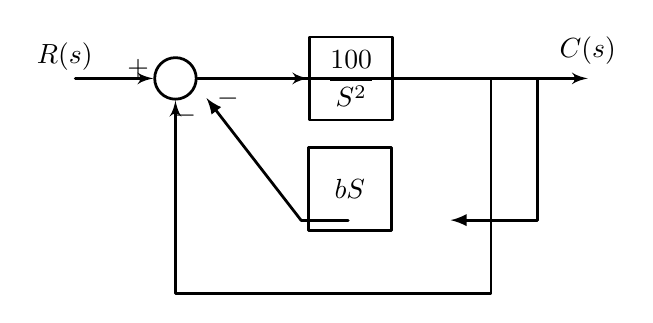
\begin{tikzpicture}
       \sbEntree{E}
       \sbCompSum*[4]{sum1}{E}{}{-}{+}{}
       \sbRelier{E}{sum1}
       \sbNomLien[0.8]{E}{$R(s)$}
       \sbBlocL[4]{a}{$\dfrac{100}{S^2}$}{sum1}
       \sbSortie[7]{S}{a}
       \sbRelier{a}{S}
       \sbNomLien[1]{S}{$C(s)$}
       \sbRenvoi[7]{a-S}{sum1}{}
       \sbDecaleNoeudy[4]{a}{S}
       \sbBlocr[-1.5]{r1}{$bS$}{S}
       \coordinate (A) at (2,0);
       \coordinate (B) at (6,-1.8);
       \draw (A) -| (B);
       \coordinate (C) at (6,-1.8);
       \coordinate (D) at (4.9,-1.8);
       \draw[-latex] (C) -- (D);
       \coordinate (E) at (3.6,-1.8);
       \coordinate (F) at (3,-1.8);
       \coordinate (G) at (1.8,-0.25);
       \draw (E) -- (F);
       \draw[-latex] (F) -- (G) node[right]{$-$};
     %\draw[-stealth] (B) -- (C)node[near end,right]{$+$};
     %\draw[-stealth] (sum.east) -- (controller.west)node[midway,above]{$e$};
     
    \end{tikzpicture}

    \vspace{1cm}

    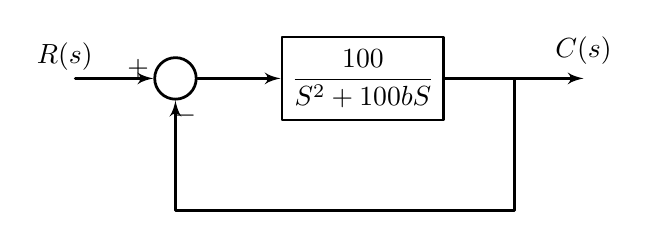
\begin{tikzpicture}
       \sbEntree{E}
       \sbCompSum*[4]{sum1}{E}{}{-}{+}{}
       \sbRelier{E}{sum1}
       \sbNomLien[0.8]{E}{$R(s)$}
       \sbBlocL[3]{a}{$\dfrac{100}{S^2+100bS}$}{sum1}
       \sbSortie[5]{S}{a}
       \sbRelier{a}{S}
       \sbNomLien[1]{S}{$C(s)$}
       \sbRenvoi[4]{a-S}{sum1}{}
     %\draw[-stealth] (B) -- (C)node[near end,right]{$+$};
     %\draw[-stealth] (sum.east) -- (controller.west)node[midway,above]{$e$};
     
    \end{tikzpicture}
    
    \vspace{1cm}

    \( \displaystyle \frac{C(s)}{R(s)} = \frac{100}{s^2 + 100bs + 100} \)

    \( \displaystyle \frac{C(s)}{R(s)} = \frac{\omega_{n}^{2}}{s^2 + 2\zeta \omega_{n}s + \omega_{n}^{2}} \)

    \vspace{2cm}

    Donde $\omega_{n}^{2}=100$ $\rightarrow$ $\omega_{n}=10$.

    \( \displaystyle 2\zeta \omega_{n} = 100b \rightarrow \zeta=5b\)

    Se tiene que el $M_{p}(\%)=5\%$.

    \( \displaystyle M_p(\%) = 100\cdot e^{- \dfrac{\zeta \pi}{\sqrt{1 - \zeta^{2}}}} = 5\% \)\\
    
    despejamos $\zeta$:

    \( \displaystyle \zeta = \sqrt{\dfrac{1}{1+ \left [ \dfrac{\pi}{\ln{M_{p}}} \right ]^{2} }} 
    = \sqrt{\dfrac{1}{1+ \left [ \dfrac{\pi}{\ln{0.05}} \right ]^{2} }} \cong 0.69 \)

    \( \displaystyle \zeta = 5b \rightarrow b=0.138 \) para que $M_{p}(\%)=5\%$

    \( \displaystyle \frac{C(s)}{R(s)} = \frac{100}{s^2 + 100bs + 100} = \frac{100}{s^2 + 13.8s + 100} \)

    \vspace{1cm}

    Ahora b para que no tenga sobreimpulso:

    \vspace{1cm}

    \( \displaystyle \frac{C(s)}{R(s)} = \frac{100}{s^2 + 100bs + 100} = \frac{\omega_{n}^{2}}{s^2 + 2\zeta \omega_{n}s + \omega_{n}^{2}} \)

    \vspace{1cm}

    Donde $\omega_{n}^{2}=100$ $\rightarrow$ $\omega_{n}=10$.

    \( \displaystyle 2\zeta \omega_{n} = 100b \rightarrow \zeta=5b\)

    Se tiene que el $M_{p}(\%)=0\%$.

    \( \displaystyle M_p(\%) = 100\cdot e^{- \dfrac{\zeta \pi}{\sqrt{1 - \zeta^{2}}}} = 0\% \)\\
    
    despejamos $\zeta$:

    \( \displaystyle \zeta = \sqrt{\dfrac{1}{1+ \left [ \dfrac{\pi}{\ln{M_{p}}} \right ]^{2} }} 
    = \sqrt{\dfrac{1}{1+ \left [ \dfrac{\pi}{\ln{0}} \right ]^{2} }} \cong 1 \)

    \( \displaystyle \zeta = 5b \rightarrow b=\frac{1}{5} \) para que $M_{p}(\%)=0\%$

    \( \displaystyle \frac{C(s)}{R(s)} = \frac{100}{s^2 + 100bs + 100} = \frac{100}{s^2 + 20s + 100} \)

    \newpage


    Para que su sobreimpulso sea de $100\%$:

    Se tiene que el $M_{p}(\%)=100\%$.

    \( \displaystyle M_p(\%) = 100\cdot e^{- \dfrac{\zeta \pi}{\sqrt{1 - \zeta^{2}}}} = 100\% \)\\
    
    despejamos $\zeta$:

    \( \displaystyle \zeta = \sqrt{\dfrac{1}{1+ \left [ \dfrac{\pi}{\ln{M_{p}}} \right ]^{2} }} 
    = \sqrt{\dfrac{1}{1+ \left [ \dfrac{\pi}{\ln{1}} \right ]^{2} }} \cong 0 \)

    \( \displaystyle \zeta = 5b \rightarrow b=0 \) para que $M_{p}(\%)=100\%$

    \( \displaystyle \frac{C(s)}{R(s)} = \frac{100}{s^2 + 100bs + 100} = \frac{100}{s^2 + 100} \)

    \newpage

    \section*{Ejercicio \# 3}


    Se debe dise\~nar sistemas de lazo cerrado, de entrada, escal\'on unitario
    determinando los valores de K y P, en algunos casos ser\'a la regi\'on del
    plano S donde se ubicar\'an las ra\'ices para que cumplan las condiciones.

    \vspace{1cm}

    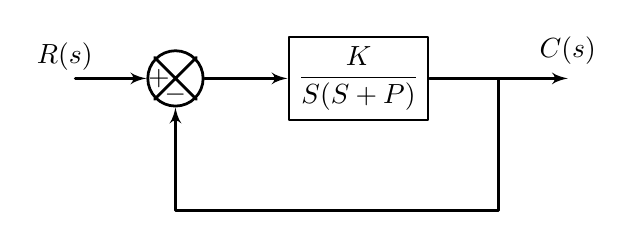
\begin{tikzpicture}
       \sbEntree{E}
       \sbCompSum[4]{sum1}{E}{}{-}{+}{}
       \sbRelier{E}{sum1}
       \sbNomLien[0.8]{E}{$R(s)$}
       \sbBlocL[3]{a}{$\dfrac{K}{S(S+P)}$}{sum1}
       \sbSortie[5]{S}{a}
       \sbRelier{a}{S}
       \sbNomLien[1]{S}{$C(s)$}
       \sbRenvoi[4]{a-S}{sum1}{}
     %\draw[-stealth] (B) -- (C)node[near end,right]{$+$};
     %\draw[-stealth] (sum.east) -- (controller.west)node[midway,above]{$e$};
     
    \end{tikzpicture}

    \begin{itemize}
      \item Datos:

        \( \displaystyle M_{p}(\%) = 15\% \)\\
        \( \displaystyle T_{s} = 6 segundos \)\\
        Determinar $K$ y $P$.

    \vspace{1cm}

    \( \displaystyle \frac{C(s)}{R(s)} = \frac{K}{s^2 + Ps + K} = \frac{\omega_{n}^{2}}{s^2 + 2\zeta \omega_{n}s + \omega_{n}^{2}} \)

    \( \displaystyle M_p(\%) = 100\cdot e^{- \dfrac{\zeta \pi}{\sqrt{1 - \zeta^{2}}}} = 15\% \)\\
    
    despejamos $\zeta$:

    \( \displaystyle \zeta = \sqrt{\dfrac{1}{1+ \left [ \dfrac{\pi}{\ln{M_{p}}} \right ]^{2} }} 
    = \sqrt{\dfrac{1}{1+ \left [ \dfrac{\pi}{\ln{0.15}} \right ]^{2} }} \cong 0.517 \)

    \vspace{1cm}

    \( \displaystyle T_{s}=4\tau=\frac{4}{\alpha}=\frac{4}{\zeta \omega_{n}}=6seconds \)

    $\omega_{n}=1.29$ 

    $\omega_{n}^{2}=1.663=K$

    $P=2\zeta \omega_{n} =2(0.517)(1.29)$

    $P=1.72$

    \(\displaystyle \frac{C(s)}{R(s)} = \frac{K}{s^2 + Ps + K} \) reemplazando
        los valores encontrados: \(\displaystyle \frac{C(s)}{R(s)}=\frac{1.663}{s^2 + 1.72s + 1.663}\)

    \end{itemize}

    \vspace{1cm}

    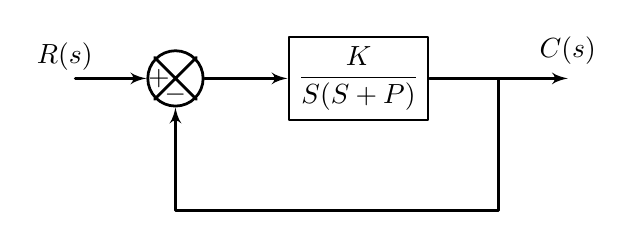
\begin{tikzpicture}
       \sbEntree{E}
       \sbCompSum[4]{sum1}{E}{}{-}{+}{}
       \sbRelier{E}{sum1}
       \sbNomLien[0.8]{E}{$R(s)$}
       \sbBlocL[3]{a}{$\dfrac{K}{S(S+P)}$}{sum1}
       \sbSortie[5]{S}{a}
       \sbRelier{a}{S}
       \sbNomLien[1]{S}{$C(s)$}
       \sbRenvoi[4]{a-S}{sum1}{}
     %\draw[-stealth] (B) -- (C)node[near end,right]{$+$};
     %\draw[-stealth] (sum.east) -- (controller.west)node[midway,above]{$e$};
     
    \end{tikzpicture}

    \begin{itemize}
      \item Datos:

        \( \displaystyle M_{p}(\%) \leq 30\% \)\\
        \( \displaystyle T_{s} \leq 6 seconds \)\\
        Determinar la regi\'on donde estar\'an las ra\'ices.

    \vspace{1cm}

    \( \displaystyle \frac{C(s)}{R(s)} = \frac{K}{s^2 + Ps + K} = \frac{\omega_{n}^{2}}{s^2 + 2\zeta \omega_{n}s + \omega_{n}^{2}} \)

    \( \displaystyle M_p(\%) = 100\cdot e^{- \dfrac{\zeta \pi}{\sqrt{1 - \zeta^{2}}}} \leq 30\% \)\\
    
    despejamos $\zeta$:

    \( \displaystyle \zeta \geq \sqrt{\dfrac{1}{1+ \left [ \dfrac{\pi}{\ln{M_{p}}} \right ]^{2} }}\)\\
    
    \(\displaystyle \zeta \geq \sqrt{\dfrac{1}{1+ \left [ \dfrac{\pi}{\ln{0.30}} \right ]^{2} }} \cong 0.517 \)

    \(\displaystyle \zeta \geq 0.358 \)

    \vspace{1cm}

    \( \displaystyle T_{s}=4\tau=\frac{4}{\alpha}=\frac{4}{\zeta \omega_{n}} \leq 6seconds \)

    $\omega_{n} \geq 1.8622$ 

    $\omega_{n}^{2} \geq 3.47=K$
      
    \vspace{0.5cm}

    $\theta \leq \arccos{(0.358)} =69.02$

    \vspace{0.5cm}

    $\alpha \geq (0.358)(1.8622)$

    $\alpha \geq 0.67$

%%grafica de las raices

\vspace{0.5cm}

    \(\displaystyle \frac{C(s)}{R(s)} = \frac{K}{s^2 + Ps + K} \) reemplazando
        los valores encontrados: \(\displaystyle \frac{C(s)}{R(s)}=\frac{3.47}{s^2 + 1.333s + 3.47}\)

    \end{itemize}

    \vspace{1cm}

    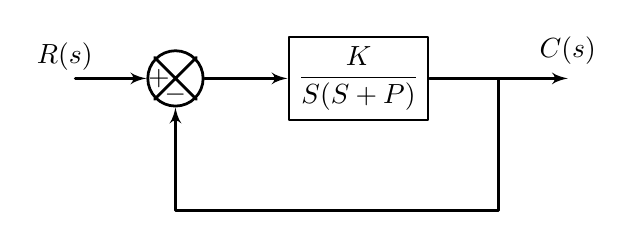
\begin{tikzpicture}
       \sbEntree{E}
       \sbCompSum[4]{sum1}{E}{}{-}{+}{}
       \sbRelier{E}{sum1}
       \sbNomLien[0.8]{E}{$R(s)$}
       \sbBlocL[3]{a}{$\dfrac{K}{S(S+P)}$}{sum1}
       \sbSortie[5]{S}{a}
       \sbRelier{a}{S}
       \sbNomLien[1]{S}{$C(s)$}
       \sbRenvoi[4]{a-S}{sum1}{}
     %\draw[-stealth] (B) -- (C)node[near end,right]{$+$};
     %\draw[-stealth] (sum.east) -- (controller.west)node[midway,above]{$e$};
     
    \end{tikzpicture}

    \begin{itemize}
      \item Datos:

        \( \displaystyle 10\% \leq M_{p}(\%) \leq 30\% \)\\
        \( \displaystyle T_{s} \leq 1 second \)\\
        Determinar la regi\'on donde estar\'an las ra\'ices.

    \vspace{1cm}

    \( \displaystyle \frac{C(s)}{R(s)} = \frac{K}{s^2 + Ps + K} = \frac{\omega_{n}^{2}}{s^2 + 2\zeta \omega_{n}s + \omega_{n}^{2}} \)

    \( \displaystyle 10\% \leq M_p(\%) = 100\cdot e^{- \dfrac{\zeta \pi}{\sqrt{1 - \zeta^{2}}}} \leq 30\% \)\\
    
    \( \displaystyle 0.1 \leq e^{- \dfrac{\zeta \pi}{\sqrt{1 - \zeta^{2}}}} \leq 0.3 \)\\
    
    despejamos $\zeta$:

    \( \displaystyle \sqrt{\dfrac{1}{1+ \left [ \dfrac{\pi}{\ln{M_{p}}} \right ]^{2} }} \geq \zeta \geq \sqrt{\dfrac{1}{1+ \left [ \dfrac{\pi}{\ln{M_{p}}} \right ]^{2} }}\)\\
    
    \( \displaystyle \sqrt{\dfrac{1}{1+ \left [ \dfrac{\pi}{\ln{0.1}} \right ]^{2} }} \geq \zeta \geq \sqrt{\dfrac{1}{1+ \left [ \dfrac{\pi}{\ln{0.3}} \right ]^{2} }}\)\\
    
    \(\displaystyle 0.6 \geq \zeta \geq 0.36 \)

    \vspace{1cm}

    \( \displaystyle T_{s}=4\tau=\frac{4}{\alpha}=\frac{4}{\zeta \omega_{n}} \leq 1second \)

        $\omega_{n_{1}} \geq 11.11$ $\rightarrow$ $\omega_{n_{1}}^{2} \geq 123.4321$
        
        $\omega_{n_{2}} \geq 6.67$ $\rightarrow$ $\omega_{n_{2}}^{2} \geq 44.4889$
      
    \vspace{0.5cm}

    $\theta \leq \arccos{(0.358)} =69.02$

    \vspace{0.5cm}

    $\alpha \geq \zeta \omega_{n}$

        $\alpha_{1} \geq (0.358)(1.8622)$ $\rightarrow$ $\alpha \geq 0.67$
        
        $\alpha_{2} \geq (0.6)(1.8622)$ $\rightarrow$ $\alpha \geq 0.67$

%%grafica de las raices

\vspace{0.5cm}

    \(\displaystyle \frac{C(s)}{R(s)} = \frac{K}{s^2 + Ps + K} \) reemplazando
        los valores encontrados: \(\displaystyle \frac{C(s)}{R(s)}=\frac{3.47}{s^2 + 1.333s + 3.47}\)

    \end{itemize}


%\begin{tikzpicture}
% 
%% Grid
%    \draw[help lines,dashed] (0,0) grid (10.25,7.25);
% 
%% Axes
%\draw[very thick,latex-latex] (0,7.75) node[left]{$\Im$}
%    |- (10,0) node[below]{$\Re$};
% 
%\draw[very thick,latex-latex] (0,-7) -- (0,0) node[above]{$$}
%    |- (-8,0) node[right]{$$};
%
%% Plot function
%\draw[ultra thick,teal] (-0.5,0) node[left,black](s0){$y(0)$}
%    -- ++(0.5,0) 
%    plot[domain=0:10,
%        samples = 50,
%        smooth]({\x}, {7*(1-exp(-\x))});
% 
%% y(infty) line 
%\draw[thick,gray] (0,7) node[left=0.1cm,black]{$y(+\infty)$} -- (10,7);
% 
%% Line with label 63%
%\draw[latex-latex] (1,0.63*7) -- (1,0) 
%    node[below]{$\tau$}
%    node[midway,fill=white]{\small $63\%$};
% 
%% Lines with label 100%
%\draw[latex-latex] (9,7) -- (9,0)
%    node[midway,fill=white]{\small $100\%$};
% 
%\end{tikzpicture}

%\begin{picture}(180,150)
%\put(20,10){\vector(0,1){150}}\put(10,20){\vector(1,0){150}}
%\multiput(15,60)(0,60){2}{\line(1,0){10}}
%\multiput(60,15)(60,0){2}{\line(0,1){10}}
%\put(60,120){\circle*{5}}\put(120,60){\circle*{5}}
%\put(60,20){\dashbox{3}(0,100){}}
%\put(120,20){\dashbox{3}(0,40){}}
%\put(20,60){\dashbox{3}(100,0){}}
%\put(20,120){\dashbox{3}(40,0){}}
%\put(70,60){\line(0,1){10}}\put(60,70){\line(1,0){10}}
%\put(60,10){\makebox(0,0){$x_1$}}
%\put(120,10){\makebox(0,0){$x_2$}}
%\put(10,60){\makebox(0,0){$y_2$}}
%\put(10,120){\makebox(0,0){$y_1$}}
%\put(90,0){\makebox(0,0){$|x_2-x_1|$}}
%\put(-5,90){\makebox(0,0){$|y_2-y_1|$}}
%\put(130,60){$(x_2,y_2)$}\put(60,130){$(x_1,y_1)$}
%\put(60,120){\line(1,-1){60}}\put(60,119.5){\line(1,-1){60}}
%\put(60,120.5){\line(1,-1){60}}\put(60,119){\line(1,-1){60}}
%\put(60,121){\line(1,-1){60}}\put(95,95){$d$}
%\end{picture}

\end{enumerate}

\end{document}
